\documentclass[tikz,border=10pt]{standalone}
\usepackage{tikz}
\usetikzlibrary{positioning}
\usepackage{tikz-feynman}
\begin{document}

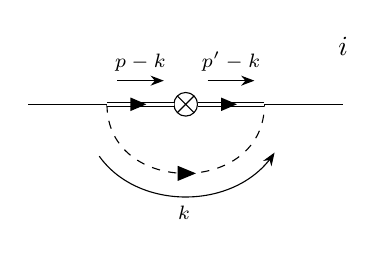
\begin{tikzpicture}[
	decuplet/.style={ % 自定义一个重子的双线
		double distance=1pt,
			postaction={decorate}, decoration={
					markings, mark=at position .6 with {
							\arrow{Triangle[angle=40:1pt 3]}
						},
				}
	}
]
	\begin{feynman}
		%% fig i
		\vertex (i1) at (0,0);
		\vertex[right =1cm  of i1] (i2);
		\vertex[right =2cm  of i1,crossed dot,anchor=center] (i3){};
		\vertex[right =3cm  of i1] (i4);
		\vertex[right =4cm  of i1] (i5);
		\node[above =0.5 of i5] {$i$};
		% 对各个顶点连线
		\diagram*{
		{
		[edge=plain]
		(i2) --[
		momentum={
				\scriptsize \(p-k\)
			}
		]  (i3) --[
		momentum={\scriptsize \(p^{\prime}-k\)}
		] (i4),
		},
		{
				[edge=plain]
				(i1) --  (i2),(i4)-- (i5),
			},
		% 介子连线
		{
		[edge= charged scalar]
		(i2) --[
		half right, momentum'={\scriptsize \(k\)}
		](i4),
		}
		};
		%% 添加重子双线
		\draw[decuplet]	 (i2) -- (i3);
		\draw[decuplet]	 (i3) -- (i4);
	\end{feynman}
\end{tikzpicture}

\end{document}

